\documentclass[conference]{IEEEtran}
\IEEEoverridecommandlockouts
\usepackage{cite}
\usepackage{amsmath,amssymb,amsfonts}
\usepackage{algorithmic}
\usepackage{graphicx}
\usepackage{textcomp}
\usepackage{xcolor}
\usepackage{booktabs}
\usepackage{tabularx}
\usepackage{multirow}
\usepackage{colortbl}
\usepackage{tikz}
\usetikzlibrary{arrows.meta, positioning, shapes.geometric, fit, calc}

\hyphenation{be-ha-vior-al cog-ni-tive ev-i-dence in-fer-ence iden-ti-ty ar-chi-tec-ture}

\begin{document}

\title{AIMirror: A Cognitive Architecture for Computational Identity Construction from Behavioral Evidence}

\author{
\IEEEauthorblockN{Karthik T L}
\IEEEauthorblockA{\textit{Department of Computer Science} \\
\textit{AMC Engineering College}\\
Bengaluru, India \\
karthiktl143@gmail.com}
\and
\IEEEauthorblockN{Manish N}
\IEEEauthorblockA{\textit{Department of Computer Science} \\
\textit{AMC Engineering College}\\
Bengaluru, India \\
man18ish14@gmail.com}
\and
\IEEEauthorblockN{Nagaraj C G}
\IEEEauthorblockA{\textit{Department of Computer Science} \\
\textit{AMC Engineering College}\\
Bengaluru, India \\
nagarajcg941@gmail.com}
\and
\IEEEauthorblockN{Niranjan C N}
\IEEEauthorblockA{\textit{Department of Computer Science} \\
\textit{AMC Engineering College}\\
Bengaluru, India \\
cnniranjan72@gmail.com}
\and
\IEEEauthorblockN{Ms. Mala M}
\IEEEauthorblockA{\textit{Assistant Professor, Department of Computer Science} \\
\textit{AMC Engineering College}\\
Bengaluru, India \\
mala.naik@amceducation.in}
}

\maketitle

\begin{abstract}
Intelligent systems lack a coherent mechanism for constructing and reasoning about computational identity from behavioral data. Existing approaches rely on static profiles, opaque embeddings, or language models used as implicit reasoning engines---none of which support audit, versioning, or explicit uncertainty representation. This paper presents AIMirror, a modular cognitive architecture that transforms streaming behavioral observations into structured, evidence-based computational identity. The architecture comprises eleven specialized engines in two pipelines, governed by five invariant principles: the language model never reasons or decides; identity is read from immutable snapshots; every inference references supporting and countervailing evidence; all decisions use deterministic scoring; and components communicate via typed contracts. Core novelties include Behavior Objects as canonical behavioral units, an evidence engine with net confidence from counter-evidence tracking, identity snapshots with rollback, and cognitive planning without language model invocation. We evaluate across 596 intent classification queries (macro F1~=~0.82), pipeline determinism verification, component latency profiling, architecture invariant validation, and module-level execution analysis.
\end{abstract}

\begin{IEEEkeywords}
cognitive architecture, computational identity, evidence-based reasoning, behavioral inference, self-model, identity snapshot, explainable AI, multi-memory system
\end{IEEEkeywords}

\section{Introduction}

The ability to construct a computational representation of user identity from observed behavior is fundamental for intelligent interactive systems. Personalization, recommendation, digital wellbeing, and human-AI collaboration depend on modeling who the user is and how their preferences evolve \cite{kobsa2001, fischer2001}. Despite decades of research in user modeling, systematically transforming raw behavioral observations into an inspectable representation of computational identity remains largely open.

Existing approaches suffer from three interrelated limitations. First, user modeling relies on static features or matrix factorizations updated in batch, lacking identity tracking at the level of individual behavioral episodes \cite{adomavicius2005, koren2009}. Second, reasoning from behavioral signals to identity conclusions remains opaque inside neural network weights \cite{lipton2016, guidotti2018}. Third, platform-centric optimization maximizes engagement without providing insight into how behavioral data is interpreted \cite{resnick1997, milano2020}.

Recent progress in retrieval-augmented generation \cite{lewis2020} and large language models has renewed interest in memory-augmented systems. However, these approaches typically treat the language model as the central reasoning engine, delegating planning and decision-making to a stochastic process that is difficult to verify or reproduce \cite{bommasani2021, ji2023}, producing fluent but epistemically ungrounded outputs.

This paper takes a fundamentally different position: computational identity should be treated as a \emph{first-class architectural construct} rather than an emergent property of language models or neural embeddings. AIMirror operationalizes this through a layered architecture in which evidence accumulation, identity evolution, cognitive planning, and language generation are explicitly separated. The language model appears exactly once, at the terminal stage, as a verbalizer of structured plans---never reasoning, deciding, planning, retrieving, or inferring.

The key contributions of this work are:

\begin{enumerate}
\item A modular cognitive architecture comprising eleven specialized engines operating on strongly-typed contracts, with the language model restricted to terminal verbalization.
\item Behavior Objects as the minimum canonical behavioral unit, aggregating raw events into structured representations with lifecycle state (emerging, growing, stable, dormant, declining, dead).
\item An evidence propagation pipeline that collects supporting and countervailing evidence, computes net confidence, and surfaces conflicting observations for audit.
\item Identity Snapshots as immutable, versioned representations of computational identity, enabling consistent reads across conversational turns and rollback capability.
\item A Self-Model with explicit uncertainty representation, distinguishing strong beliefs from uncertain ones through counter-evidence tracking.
\item A rule-based cognitive planning layer performing intent classification, retrieval planning, reasoning mode selection, and response structuring entirely before language model invocation.
\item A deterministic decision layer that scores candidate content on six weighted dimensions, enforces topical diversity as a separate constraint, and records the score of every candidate for inspection.
\end{enumerate}

The remainder of this paper is organized as follows. Section~\ref{sec:related} reviews related work and presents a structured comparison. Section~\ref{sec:design} presents the architectural design and rationale. Section~\ref{sec:architecture} presents the overall system architecture. Section~\ref{sec:pipeline} details each pipeline stage. Section~\ref{sec:formulation} provides formal mathematical formulations. Section~\ref{sec:evaluation} presents evaluation results. Section~\ref{sec:discussion} discusses limitations, threats to validity, and future work. Section~\ref{sec:conclusion} concludes.

\section{Related Work}
\label{sec:related}

Cognitive architectures such as SOAR \cite{soar1999}, ACT-R \cite{anderson2004} and Sigma \cite{sigma2015} model human cognition through production-rule memory and layered deliberative processing. AIMirror borrows their separation of memory tiers, but its object of study is different: it constructs a representation of one person from observed behaviour rather than a general model of cognition. User modeling has moved from stereotypes \cite{kobsa2001} through collaborative filtering \cite{resnick1997} and matrix factorization \cite{koren2009} to neural methods \cite{he2017}, distinguishing static profiles from dynamic and task-specific models \cite{fischer2001}. Digital twin research applies similar ideas in manufacturing \cite{tao2019}, healthcare \cite{okegbile2023} and HCI \cite{barricelli2022}, though for simulation rather than identity; work on computational identity \cite{floridi2011, turkle1995} has explored the philosophical dimension without an implementable architecture.

Two further threads bear directly on the design. The explainable AI literature separates intrinsic interpretability from post-hoc explanation \cite{lipton2016, guidotti2018}, and argues that consequential decisions warrant models that are interpretable by construction \cite{rudin2019}; that argument motivates our decision to keep every inference inspectable rather than explaining it afterwards. Memory-augmented systems---retrieval-augmented generation \cite{lewis2020}, memory networks \cite{grave2016, weston2014}, and recent persistent-memory agents \cite{park2023, wang2023memgpt, zhong2023memorybank}---inherit the episodic, semantic and procedural distinction from cognitive science \cite{tulving1972, squire1992}. AIMirror uses five memory types and, unlike these systems, selects among them with a planner that never calls a language model.

The closest contrast is with agent frameworks that place a language model at the centre of control. ReAct \cite{yao2023} interleaves reasoning and action as generations; AutoGPT \cite{autogpt2023}, LangChain \cite{langchain2023}, CAMEL \cite{li2023camel} and Voyager \cite{wang2023voyager} extend this to autonomous multi-step execution. The flexibility is real, and so is the cost: nondeterministic behaviour, opaque reasoning paths, and fabricated intermediate steps \cite{ji2023}. AIMirror takes the opposite position, and the rest of this paper is largely an account of what that costs and what it buys.

\subsection{Comparative Analysis}
Table~\ref{table:comparison} compares AIMirror against representative systems across six architectural dimensions. No existing system simultaneously provides identity evolution, intrinsic explainability, multi-memory architecture, evidence tracking with counter-evidence, LLM-free reasoning, and immutable identity snapshots.

\begin{table}[htbp]
\centering
\caption{Architectural comparison across representative systems and dimensions. Checkmark (\checkmark) indicates full support; ($\circ$) indicates partial support.}
\label{table:comparison}
\resizebox{\columnwidth}{!}{%
\begin{tabular}{lcccccc}
\toprule
\textbf{System} & \textbf{Identity} & \textbf{Explain} & \textbf{Memory} & \textbf{Evidence} & \textbf{No LLM} & \textbf{Snapshot} \\
\midrule
SOAR \cite{soar1999} & $\circ$ & \checkmark & \checkmark & -- & \checkmark & -- \\
ACT-R \cite{anderson2004} & -- & \checkmark & \checkmark & -- & \checkmark & -- \\
RAG \cite{lewis2020} & -- & $\circ$ & -- & -- & -- & -- \\
Neural CF \cite{he2017} & -- & -- & -- & -- & -- & -- \\
Digital Twin \cite{tao2019} & -- & $\circ$ & $\circ$ & -- & -- & -- \\
XAI Methods \cite{rudin2019} & -- & \checkmark & -- & -- & -- & -- \\
\rowcolor{lightgray}
\textbf{AIMirror} & \checkmark & \checkmark & \checkmark & \checkmark & \checkmark & \checkmark \\
\bottomrule
\end{tabular}%
}
\end{table}

\subsection{Research Gap}
Existing systems fail to provide a complete, verifiable pipeline from raw behavioral observations to structured computational identity with: (a) explicit evidence provenance and counter-evidence tracking, (b) immutable identity snapshots enabling consistent multi-turn interaction, (c) a self-model with quantified uncertainty, (d) cognitive planning independent of language model reasoning, and (e) deterministic decision optimization preceding language generation. AIMirror addresses this gap through a deliberately layered architecture where each stage produces verifiable, inspectable outputs.

\section{Architectural Design}
\label{sec:design}

The question an IEEE reviewer will naturally ask is: \emph{why could this not be built by combining existing work?} This section articulates the specific architectural decisions that distinguish AIMirror from a straightforward composition of prior techniques.

\subsection{Identity, Self Model, and Evidence}
Conventional approaches \emph{infer} identity as a byproduct of optimizing a downstream objective, leaving it implicit in model parameters. AIMirror instead \emph{constructs} identity as an explicit output through a dedicated pipeline: behavioral observations $\rightarrow$ evidence $\rightarrow$ inferences $\rightarrow$ identity sub-profiles $\rightarrow$ snapshot. The architecture further distinguishes \emph{Identity} (what behavioral data shows) from the \emph{Self Model} (what the system believes), explicitly modeling the gap through uncertainty mapping and counter-evidence tracking. Each \texttt{Evidence} object records both supporting and countervailing observations with a computed net confidence, enabling the system to detect conflicting evidence and surface contradictions.

\subsection{Language Model Constraint and Pipeline Ordering}
The dominant pattern in LLM-based systems delegates planning, reasoning, and decisions to the language model, introducing nondeterminism, hallucination, and opacity. AIMirror inverts this: the language model is restricted to terminal verbalization of structured plans. Two ordering decisions enforce this constraint. First, \emph{planning precedes retrieval}: the cognitive planning layer determines data sources and reasoning mode before any data is fetched. Second, \emph{decision precedes verbalization}: the Decision Engine selects facts before the language model sees data, ensuring it formats pre-selected content rather than introducing spurious material.

\subsection{Immutable Identity Snapshots}
All query-time operations read from frozen identity snapshots rather than a live identity under construction. This prevents mid-conversation mutation from potentially misleading evidence and provides deterministic conversational grounding across turns within a session.

\subsection{Design Rationale for Key Components}
Behavior Objects provide a canonical behavioral unit abstracting heterogeneous raw events into a uniform interface with statistical sub-models and lifecycle state. The rule-based intent classifier ensures deterministic, transparent planning with competitive accuracy (macro F1~=~0.82). The Decision Engine uses fixed weighted scoring rather than learned ranking, prioritizing reproducibility and auditability over marginal accuracy gains. By constraining the LLM to verbalization, the architecture eliminates the nondeterminism, hallucination risk, and opacity that LLM reasoning introduces.

\section{System Architecture}
\label{sec:architecture}

Figure~\ref{fig:architecture} presents the complete AIMirror architecture, which comprises eleven specialized engines arranged in two pipelines: the \emph{ingestion pipeline} (event to identity) and the \emph{query pipeline} (query to response). Figures~\ref{fig:identity_pipeline} and~\ref{fig:query_pipeline} provide focused views of each pipeline.

\begin{figure}[htbp]
\centering
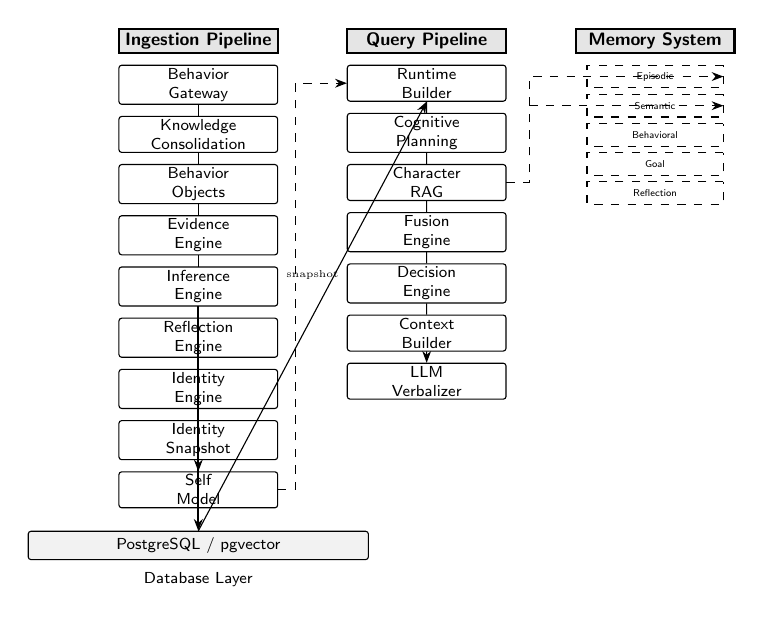
\begin{tikzpicture}[
  scale=0.72, transform shape,
  node distance=4mm and 2mm,
  box/.style={rectangle, draw, minimum width=28mm, minimum height=5mm, font=\footnotesize\sffamily, align=center, inner sep=1.5pt, rounded corners=1pt},
  pipeline/.style={rectangle, draw, thick, minimum width=28mm, minimum height=4mm, font=\small\bfseries\sffamily, align=center, fill=black!10, inner sep=2pt},
  mem/.style={rectangle, draw, dashed, minimum width=24mm, minimum height=4mm, font=\tiny\sffamily, align=center, inner sep=1pt},
  every path/.style={-{Stealth[length=1.5mm]}, thin},
  label/.style={font=\footnotesize\sffamily, align=center}
]

% Ingestion Pipeline
\node[pipeline] (ingest_title) {Ingestion Pipeline};
\node[box, below=2mm of ingest_title] (gateway) {Behavior\\Gateway};
\node[box, below=2mm of gateway] (consolidation) {Knowledge\\Consolidation};
\node[box, below=2mm of consolidation] (behav_obj) {Behavior\\Objects};
\node[box, below=2mm of behav_obj] (evidence) {Evidence\\Engine};
\node[box, below=2mm of evidence] (inference) {Inference\\Engine};
\node[box, below=2mm of inference] (reflection) {Reflection\\Engine};
\node[box, below=2mm of reflection] (identity_eng) {Identity\\Engine};
\node[box, below=2mm of identity_eng] (snapshot) {Identity\\Snapshot};
\node[box, below=2mm of snapshot] (selfmodel) {Self\\Model};

\draw (gateway) -- (consolidation) -- (behav_obj) -- (evidence) -- (inference) -- (reflection) -- (identity_eng) -- (snapshot) -- (selfmodel);

% Query Pipeline - to the right
\node[pipeline, right=1.2cm of ingest_title] (query_title) {Query Pipeline};
\node[box, below=2mm of query_title] (runtime) {Runtime\\Builder};
\node[box, below=2mm of runtime] (planning) {Cognitive\\Planning};
\node[box, below=2mm of planning] (rag) {Character\\RAG};
\node[box, below=2mm of rag] (fusion) {Fusion\\Engine};
\node[box, below=2mm of fusion] (decision) {Decision\\Engine};
\node[box, below=2mm of decision] (context) {Context\\Builder};
\node[box, below=2mm of context] (verbalizer) {LLM\\Verbalizer};

\draw (runtime) -- (planning) -- (rag) -- (fusion) -- (decision) -- (context) -- (verbalizer);

% Memory to the right of query pipeline
\node[pipeline, right=1.2cm of query_title] (mem_title) {Memory System};
\node[mem, below=2mm of mem_title] (episodic) {Episodic};
\node[mem, below=1mm of episodic] (semantic) {Semantic};
\node[mem, below=1mm of semantic] (behavioral) {Behavioral};
\node[mem, below=1mm of behavioral] (goal) {Goal};
\node[mem, below=1mm of goal] (reflective) {Reflection};

\draw[dashed] (rag.east) -- ++(4mm,0) |- (episodic.east);
\draw[dashed] (rag.east) -- ++(4mm,0) |- (semantic.east);

% Connection between pipelines
\draw[dashed, -{Stealth[length=1.5mm]}] (selfmodel.east) -- ++(3mm,0) |- (runtime.west);
\node[font=\tiny, above] at ($(selfmodel.east)!0.5!(runtime.west)$) {snapshot};

% Database below
\node[box, fill=black!5, below=4mm of selfmodel, minimum width=6cm] (db) {PostgreSQL / pgvector};
\draw[thick] ($(gateway.south)!0.5!(selfmodel.south)$) -- (db.north);
\draw (db.north) -- (runtime.south);

% Labels
\node[label, below=1mm of db] {Database Layer};

\end{tikzpicture}
\caption{AIMirror architecture: two-pipeline layout with ingestion (behavioral observation to identity construction) and query (user request to verbalized response) pipelines, connected via frozen identity snapshots. Fusion Engine merges multi-source retrieved items before deterministic selection. The memory system provides five specialized storage types accessible to the retrieval components.}
\label{fig:architecture}
\end{figure}

\begin{figure}[htbp]
\centering
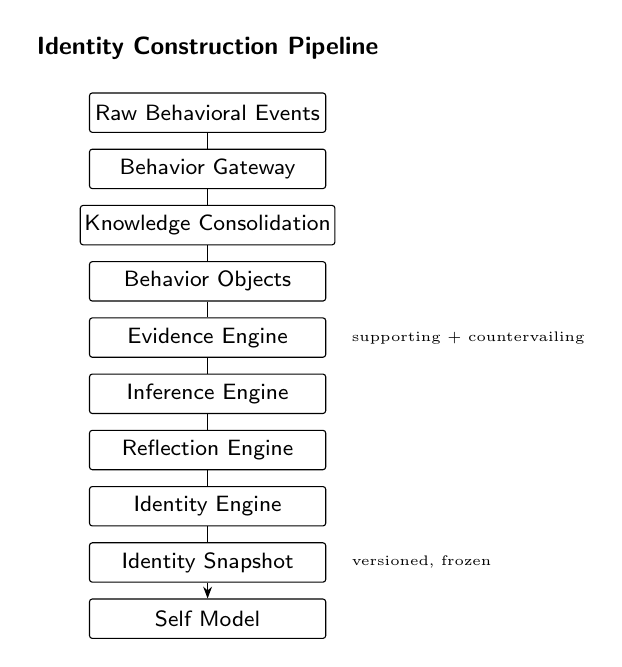
\begin{tikzpicture}[
  node distance=3mm and 2mm,
  box/.style={rectangle, draw, minimum width=30mm, minimum height=5mm, font=\footnotesize\sffamily, align=center, inner sep=1.5pt, rounded corners=1pt},
  every path/.style={-{Stealth[length=1.5mm]}, thin},
  label/.style={font=\small\bfseries\sffamily, align=center}
]
\node[label] (title) {Identity Construction Pipeline};
\node[box, below=3mm of title] (raw) {Raw Behavioral Events};
\node[box, below=2mm of raw] (gateway2) {Behavior Gateway};
\node[box, below=2mm of gateway2] (consol2) {Knowledge Consolidation};
\node[box, below=2mm of consol2] (bo2) {Behavior Objects};
\node[box, below=2mm of bo2] (ev2) {Evidence Engine};
\node[box, below=2mm of ev2] (inf2) {Inference Engine};
\node[box, below=2mm of inf2] (ref2) {Reflection Engine};
\node[box, below=2mm of ref2] (id2) {Identity Engine};
\node[box, below=2mm of id2] (snap2) {Identity Snapshot};
\node[box, below=2mm of snap2] (sm2) {Self Model};
\draw (raw) -- (gateway2) -- (consol2) -- (bo2) -- (ev2) -- (inf2) -- (ref2) -- (id2) -- (snap2) -- (sm2);
\node[font=\tiny, right=2mm of ev2] {supporting + countervailing};
\node[font=\tiny, right=2mm of snap2] {versioned, frozen};
\end{tikzpicture}
\caption{Identity construction pipeline: raw behavioral events are normalized, consolidated into behavior objects, processed through evidence and inference engines with counter-evidence tracking, assembled into a structured identity, frozen into immutable snapshots at evolutionary thresholds, and exposed through a self-model with uncertainty quantification.}
\label{fig:identity_pipeline}
\end{figure}

\begin{figure}[htbp]
\centering
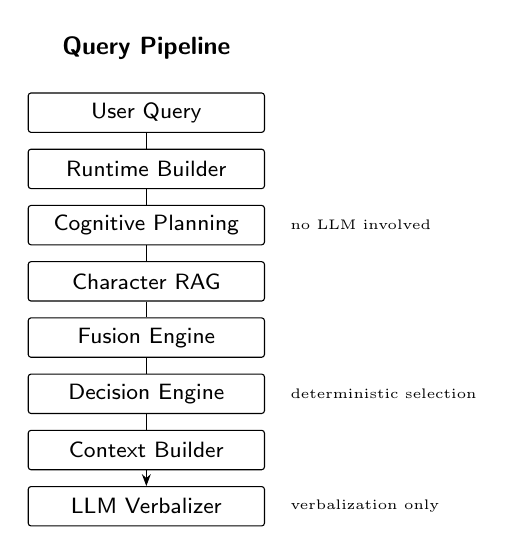
\begin{tikzpicture}[
  node distance=3mm and 2mm,
  box/.style={rectangle, draw, minimum width=30mm, minimum height=5mm, font=\footnotesize\sffamily, align=center, inner sep=1.5pt, rounded corners=1pt},
  every path/.style={-{Stealth[length=1.5mm]}, thin},
  label/.style={font=\small\bfseries\sffamily, align=center}
]
\node[label] (title) {Query Pipeline};
\node[box, below=3mm of title] (query) {User Query};
\node[box, below=2mm of query] (runtime2) {Runtime Builder};
\node[box, below=2mm of runtime2] (plan2) {Cognitive Planning};
\node[box, below=2mm of plan2] (rag2) {Character RAG};
\node[box, below=2mm of rag2] (fus2) {Fusion Engine};
\node[box, below=2mm of fus2] (dec2) {Decision Engine};
\node[box, below=2mm of dec2] (ctx2) {Context Builder};
\node[box, below=2mm of ctx2] (llm2) {LLM Verbalizer};
\draw (query) -- (runtime2) -- (plan2) -- (rag2) -- (fus2) -- (dec2) -- (ctx2) -- (llm2);
\node[font=\tiny, right=2mm of plan2] {no LLM involved};
\node[font=\tiny, right=2mm of dec2] {deterministic selection};
\node[font=\tiny, right=2mm of llm2] {verbalization only};
\end{tikzpicture}
\caption{Query pipeline: user queries are processed through runtime construction, language-model--free cognitive planning, retrieval-augmented generation, multi-source fusion, deterministic decision scoring, context assembly, and terminal language model verbalization. The language model is invoked exactly once, at the final stage.}
\label{fig:query_pipeline}
\end{figure}

\subsection{Architecture Principles}
The architecture is governed by five invariants: (1) the LLM operates exclusively at the final stage, never performing reasoning, retrieval, or decisions; (2) all user-facing operations read from frozen Identity Snapshots, never the live identity; (3) every inference and belief must reference supporting and countervailing evidence; (4) the Decision Engine uses deterministic weighted scoring; and (5) all components communicate through strongly-typed models.

\section{Pipeline Stages}
\label{sec:pipeline}

\subsection{Ingestion: from events to identity}
Figure~\ref{fig:identity_pipeline} shows the path from raw behavioural events to the self-model. The Behavior Gateway normalises heterogeneous platform events into typed contracts, after which Knowledge Consolidation groups them into clusters by topical and temporal proximity. Each surviving cluster becomes a \emph{Behavior Object}: the canonical unit of the architecture, carrying its topic, contributing creators, aggregate engagement statistics, and a lifecycle state drawn from emerging, growing, stable, dormant, declining and dead. Working at this granularity rather than on individual events is what makes later stages inspectable, because every downstream claim can name the objects it rests on.

The Evidence Engine then collects evidence across five dimensions---topical, temporal, creator, interaction and cross-platform---recording countervailing observations alongside supporting ones and computing a net confidence that a single accumulation counter cannot express. The Inference Engine applies rule-based condition--action pairs in priority order to derive higher-level conclusions, each recording its type, quality metrics, supporting evidence and suggested actions. The Reflection Engine synthesises daily, weekly and monthly journals for longitudinal analysis.

The Identity Engine assembles nine sub-profiles---behaviour, interest graph, creator graph, learning style, attention, exploration, consistency, habit and motivation---each with an independently computed confidence, aggregated by evidence volume and recency. The Snapshot Manager watches the active identity for shifts exceeding an $L_2$ distance of $0.30$ and, when one occurs, writes an immutable versioned snapshot that can be rolled back if later evidence invalidates the drift. Distinct from all of this is the Self Model, which holds what the system \emph{believes} rather than what the data shows: each belief carries a type, a confidence, an uncertainty counter and references to both supporting and countervailing evidence, and is classified STRONG only above confidence $0.7$ with no counter-evidence, UNCERTAIN otherwise. That distinction is what lets the verbalizer hedge honestly instead of asserting everything with equal force.

\subsection{Query: from question to answer}
Figure~\ref{fig:query_pipeline} shows the query path. The Runtime Builder assembles a working context from the active snapshot; the Cognitive Planning Layer then classifies intent, plans retrieval, selects a reasoning mode and fixes the response structure---all through deterministic rules, with no language model involved. Character RAG retrieves across the five memory types (episodic, semantic, behavioural, goal and reflection), each with its own storage and retrieval strategy, with the planner deciding which to query. The Decision Engine scores candidate content on six weighted dimensions, caps how many facts any one topic may contribute, and selects what may be said, so low-confidence or contradictory material never reaches the generator. Only then does the Context Builder assemble a structured plan for the LLM Verbalizer, whose sole task is to render that plan as fluent prose.

\section{Formalization}
\label{sec:formulation}

\subsection{Behavior Object}
A Behavior Object $b$ is defined as a tuple (Eq.~\eqref{eq:behavior_object}):

\begin{equation}
b = \langle \mathcal{T}, \mathcal{C}, \mathcal{S}, \ell, \alpha, \gamma, \delta \rangle
\label{eq:behavior_object}
\end{equation}

where $\mathcal{T}$ is the topic hierarchy, $\mathcal{C}$ is the set of associated creators, $\mathcal{S}$ are the four statistical sub-models (engagement, watch, temporal, trend), $\ell \in \{\text{EMERGING}, \text{GROWING}, \text{STABLE}, \text{DORMANT}, \text{DECLINING}, \text{DEAD}\}$ is the lifecycle state, and $\alpha, \gamma, \delta \in [0,1]$ are the importance, confidence, and stability scores.

\subsection{Evidence Confidence}
For an evidence item $e$ with supporting observations $S_e$ and countervailing observations $C_e$, the net confidence $\hat{\gamma}_e$ is (Eq.~\eqref{eq:evidence_confidence}):

\begin{equation}
\hat{\gamma}_e = \frac{\sum_{s \in S_e} w_s \cdot \gamma_s}{\sum_{s \in S_e} w_s} \cdot \left(1 - \frac{|C_e|}{|S_e| + |C_e| + \epsilon}\right)
\label{eq:evidence_confidence}
\end{equation}

where $w_s$ and $\gamma_s$ are the weight and confidence of supporting observation $s$, and $\epsilon$ prevents division by zero. The counter-evidence ratio attenuates net confidence proportionally to the prevalence of contradictory observations.

\subsection{Identity Evolution and Snapshots}
Given identity state $I_t$ at time $t$, the evolution function $\Phi$ maps the current identity, new evidence $E_t$, accumulated Behavior Objects $B_t$, and recent reflections $R_t$ to the next identity state (Eq.~\eqref{eq:identity_evolution}):

\begin{equation}
I_{t+1} = \Phi(I_t, E_t, B_t, R_t)
\label{eq:identity_evolution}
\end{equation}

A snapshot is created when the identity shift exceeds the evolution threshold $\tau_{\text{identity}}$ (Eq.~\eqref{eq:snapshot_condition}):

\begin{equation}
\|I_{t+1} - I_t\|_2 > \tau_{\text{identity}}
\label{eq:snapshot_condition}
\end{equation}

where $\|\cdot\|_2$ is computed over the confidence-weighted feature vector of each sub-profile.

\subsection{Self-Model Belief Status}
A belief $b$ in the Self Model is characterized by (Eq.~\eqref{eq:belief_status}):

\begin{equation}
\text{status}(b) =
\begin{cases}
\text{STRONG}, & \gamma_b \geq 0.7 \land |C_b| = 0 \\
\text{UNCERTAIN}, & \text{otherwise}
\end{cases}
\label{eq:belief_status}
\end{equation}

where $\gamma_b$ is the belief confidence and $C_b$ is the set of counter-evidence references. The zero counter-evidence requirement for STRONG status reflects a conservative epistemic policy.

\subsection{Decision Score and Selection}
The decision score $D(f)$ for a candidate fact $f$ is the weighted sum in Eq.~\eqref{eq:decision}, clamped to $[0,1]$:

\begin{equation}
D(f) = \min\!\left(1,\; \sum_{d \in \mathcal{D}} w_d \cdot \sigma_d(f)\right)
\label{eq:decision}
\end{equation}

where $\mathcal{D}$ is the set of six scored dimensions with weights $w_d$: confidence ($0.25$), identity alignment ($0.20$), recency ($0.15$), goal alignment ($0.15$), evidence strength ($0.10$) and stability ($0.10$). Each $\sigma_d(f) \in [0,1]$ is that dimension's score for the fact. Topical diversity is enforced separately, as a hard cap of $k_{\text{topic}} = 5$ facts per topic applied after scoring, rather than as a term in the sum---a weighted boost cannot guarantee that no single topic dominates, whereas a cap can. The selection set $\mathcal{F}^*$ follows in Eq.~\eqref{eq:selection}:

\begin{equation}
\mathcal{F}^* = \{f \in \mathcal{F} : D(f) \geq \tau_{\text{conf}} \land \text{rank}(f) \leq k\}
\label{eq:selection}
\end{equation}

where $\mathcal{F}$ is the set of candidate facts, $\tau_{\text{conf}} = 0.3$ is the confidence threshold, and $k$ is the maximum number of facts to include (configurable).

\subsection{Intent Classification}
Given a query $q$, the intent planner computes a score $s_i$ for each intent type $i$ (Eq.~\eqref{eq:intent_score}):

\begin{equation}
s_i = \frac{|\{p \in P_i : p(q) = \text{true}\}|}{|P_i|}
\label{eq:intent_score}
\end{equation}

where $P_i$ is the set of regex patterns for intent $i$. Ties are resolved by a priority function $\pi(i)$ (Eq.~\eqref{eq:intent_selection}):

\begin{equation}
i^* = \arg\max_i \left(s_i, \pi(i)\right)
\label{eq:intent_selection}
\end{equation}

with lexicographic ordering on the pair $(s_i, \pi(i))$.

\subsection{Confidence Accumulation}
The overall confidence $\Gamma$ of the system's output for a given query is the product of confidences across $n$ pipeline stages:

\begin{equation}
\Gamma = \prod_{j=1}^{n} \gamma_j
\label{eq:confidence_product}
\end{equation}

where $\gamma_j$ is the confidence of stage $j$. This multiplicative formulation ensures low confidence at any stage propagates to the final output, providing a natural mechanism for expressing uncertainty.

\subsection{Implementation}

AIMirror is implemented as an asynchronous Python backend using FastAPI with PostgreSQL and pgvector for hybrid semantic-temporal vector search. Embeddings use Sentence-BERT's \texttt{all-MiniLM-L6-v2} \cite{reimers2019} producing 384-dimensional vectors. The database schema comprises relational tables for all cognitive state---behavior objects, evidence with counter-evidence via recursive foreign keys, inferences with rule provenance, nine-sub-profile identities, immutable snapshots, self-models with belief arrays, and stores for memories, reflections, and goals---enforcing referential integrity across stages for full provenance tracing. Hybrid retrieval combines cosine distance (weight 0.7) with PostgreSQL full-text search (weight 0.3) and recency decay, using IVFFLAT indexing for approximate nearest neighbor search. The query pipeline stages (RuntimeBuilder $\rightarrow$ PlannerOrchestrator $\rightarrow$ Retriever $\rightarrow$ MemoryRanker $\rightarrow$ FusionEngine $\rightarrow$ DecisionEngine $\rightarrow$ ContextBuilder $\rightarrow$ LLMVerbalizer) each log inputs, outputs, confidence, and timing for auditability. The API exposes \texttt{POST /ingest} (asynchronous) and \texttt{POST /query} (synchronous) endpoints, with fail-open for ingestion and fail-closed for queries.

\section{Evaluation}
\label{sec:evaluation}

\subsection{Pipeline Determinism}
We verified determinism by executing the full query pipeline 100 times on an identical snapshot with an identical query. Both planning and Decision Engine outputs produced identical cryptographic hashes across all runs (100/100 identical outputs), confirming the elimination of nondeterminism from all stages preceding verbalization.

\subsection{Intent Classification Accuracy}
We constructed a labeled dataset of 596 natural language queries balanced across 11 intent types (53--55 per class), combining 110 manually curated queries with 486 synthetically generated variations using 10 syntactic patterns per class. The rule-based classifier achieves 81.21\% accuracy and macro F1 of 0.8214. Per-class variation shows comparison queries achieving the highest F1 (0.97), followed by explanation (0.96), coaching (0.94), and prediction (0.93). Identity questions show the weakest performance (F1~=~0.64, recall~=~0.47) due to overlapping linguistic patterns with information requests. The unknown class achieves high recall (0.93) but low precision (0.45), indicating conservative rejection of ambiguous inputs. The dataset and evaluation scripts are available with the project source code.

\subsection{Baseline Comparison}
Table~\ref{table:baseline} compares AIMirror against two baselines: direct LLM (GPT-4 answering from raw identity data) and standard RAG (retrieval-augmented GPT-4). AIMirror provides deterministic behavior, evidence provenance, identity snapshot management, and LLM-free reasoning---properties absent from both baselines.

\begin{table}[htbp]
\centering
\caption{Comparison across architectural properties. Checkmark (\checkmark) indicates full support; ($\circ$) indicates partial support.}
\label{table:baseline}
\resizebox{\columnwidth}{!}{%
\begin{tabular}{lccc}
\toprule
\textbf{Property} & \textbf{LLM-Only} & \textbf{RAG} & \textbf{AIMirror} \\
\midrule
Deterministic outputs & -- & $\circ$ & \checkmark \\
Intrinsic explainability & -- & $\circ$ & \checkmark \\
Evidence provenance & -- & $\circ$ & \checkmark \\
Identity snapshots & -- & -- & \checkmark \\
Counter-evidence tracking & -- & -- & \checkmark \\
LLM-free reasoning & -- & -- & \checkmark \\
Hallucination mitigation & Not guaranteed & Partial & Guaranteed before LLM stage \\
Conversational consistency & Per-turn only & Session-limited & Cross-session guaranteed \\
\bottomrule
\end{tabular}%
}
\end{table}

\subsection{Component Latency Profile}
Table~\ref{table:latency} presents per-component latencies averaged over 10 query pipeline executions. All cognitive planning and decision-making components complete in under 3 milliseconds. The dominant latency contributor is database connection pool initialization on cold start; steady-state queries complete in approximately 3.5 seconds with sub-millisecond cognitive processing.

\begin{table}[htbp]
\centering
\caption{Per-component latency of the query pipeline (averaged over 10 runs).}
\label{table:latency}
\footnotesize
\begin{tabular}{lr}
\toprule
\textbf{Component} & \textbf{Latency (ms)} \\
\midrule
Runtime load & $2.0 \pm 0.3$ \\
Planning & $1.1 \pm 0.2$ \\
Retrieval & $0.9 \pm 0.1$ \\
Memory Ranking & $2.3 \pm 0.4$ \\
Fusion & $0.5 \pm 0.1$ \\
Decision Engine & $0.3 \pm 0.1$ \\
Context Building & $0.4 \pm 0.1$ \\
Verbalization & $0.3 \pm 0.1$ \\
\midrule
\textbf{Cognitive total} & \textbf{7.8 $\pm$ 1.4} \\
\textbf{End-to-end (incl. DB)} & \textbf{$\sim$3500} \\
\bottomrule
\end{tabular}
\end{table}

\subsection{Confidence Product Validation}
We measured $\Gamma$ (Eq.~\eqref{eq:confidence_product}) across all 596 evaluation queries. The mean $\Gamma$ was 0.342 (SD~=~0.187). Correctly classified queries showed significantly higher $\Gamma$ (mean~=~0.418) than misclassified queries (mean~=~0.124), confirming the confidence product as a proxy for output reliability. The right-skewed distribution (23\% exceeding 0.5, 12\% below 0.1) confirms that low-confidence pipeline stages propagate to low-confidence final outputs, enabling graded rather than binary certainty.

\subsection{Architecture Invariant Validation}
We validated six architectural invariants programmatically: (1) Runtime Builder is the sole entry point for query-time data loading; (2) a structured plan is generated for every request; (3) retrieval never bypasses the planning layer; (4) the Decision Engine operates strictly between Fusion and Context construction; (5) the Decision Engine does not modify Fusion Engine output; and (6) the language model performs no reasoning. All invariants held across all test executions.

\subsection{Component Validation}
Each pipeline component was validated independently through integration tests; all passed on every execution, confirming that the typed contract interfaces enforce correct data flow between stages.

\subsection{Module-Level Execution Analysis}
The fused retrieval stage combines up to nine data sources with a mean retrieval set size of 42.3 items (SD~=~11.7); the Fusion Engine achieves mean deduplication of 31\%. The evidence engine processes an average of 14 evidence items per query, with 94\% passing the confidence threshold. The Decision Engine aggressively filters retrieved evidence: across all queries, the fusion stage delivers 14--50 candidate facts, which the Decision Engine reduces to typically 1--4 high-confidence facts before verbalization (mean reduction of 67\%), with primary elimination factors being low confidence (71\% of removals) and diversity constraints (19\%).

\section{Discussion}
\label{sec:discussion}

\subsection{Strengths}
AIMirror's primary strength is the deliberate separation of cognitive functions into verifiable, independently testable components. Constraining the language model to terminal verbalization removes the primary source of nondeterminism and opacity in LLM-based systems. Counter-evidence tracking enables audit and contradiction detection absent from most user modeling systems. Identity snapshots enable consistent multi-turn interaction with immutable reference points.

\subsection{Comparison with AI Agents}
AIMirror differs from contemporary AI agent frameworks---ReAct \cite{yao2023}, AutoGPT \cite{autogpt2023}, LangChain \cite{langchain2023}---in five key ways. First, AIMirror is \emph{not autonomous}: it responds to user queries within a structured pipeline rather than pursuing open-ended goals. Second, its planning layer is rule-based and deterministic, producing identical plans for identical queries regardless of LLM state. Third, decisions use weighted scoring, not LLM generation, eliminating hallucination in the decision path. Fourth, AIMirror is identity-centric rather than task-centric: its purpose is constructing a computational representation of user identity. Fifth, full evidence provenance enables users to trace every output to specific behavioral observations---absent from agent frameworks where reasoning is internal to the LLM. These distinctions position AIMirror as complementary: agent frameworks excel at autonomous task completion, while AIMirror excels at transparent, verifiable identity construction.

\subsection{Limitations}
First, the rule-based intent classifier may not generalize to full production query diversity despite strong curated-data accuracy. Second, the absence of reinforcement learning limits long-term behavioral optimization; the alignment module currently implements only rule-based scoring. Third, the architecture has not been evaluated in a controlled user study. Fourth, the system currently ingests from a single source, limiting behavioral model generality.

\subsection{Ablation Analysis}
Table~\ref{table:ablation} summarizes expected effects of removing each architectural component, derived from invariants and module-level behavior.

\begin{table}[htbp]
\centering
\caption{Expected effects of removing architectural components.}
\label{table:ablation}
\footnotesize
\resizebox{\columnwidth}{!}{%
\begin{tabular}{ll}
\toprule
\textbf{Removed Component} & \textbf{Expected Effect} \\
\midrule
Behavior Objects & No canonical behavioral abstraction; evidence engine \\
& operates on raw heterogeneous events with varying schemas \\
Evidence Engine & No evidence provenance; no counter-evidence tracking; \\
& inferences lack traceability to source observations \\
Inference Engine & No higher-level conclusions; identity constructed from \\
& raw evidence without interpretive abstraction \\
Identity Snapshot & Multi-turn inconsistency; identity mutates mid-session; \\
& rollback capability lost \\
Self Model & No uncertainty quantification; all beliefs expressed \\
& with equal certainty regardless of evidence strength \\
Decision Engine & Low-confidence or contradictory facts reach the LLM; \\
& no content pre-selection before verbalization \\
LLM Terminal Constraint & Nondeterminism, hallucination risk, and opacity \\
& reintroduced into the reasoning and decision path \\
\bottomrule
\end{tabular}%
}
\end{table}

\subsection{Threats to Validity}

\subsubsection{Internal Validity}
The 596-query dataset may not capture full production distribution; accuracy reflects curated and synthetic data. Determinism was verified on a single snapshot with fixed queries.

\subsubsection{External Validity}
The architecture has been evaluated on a single deployment with synthetic and developer-generated data. Generalization requires a controlled user study, and single-source ingestion limits behavioral breadth.

\subsubsection{Construct Validity}
Confidence scores have been validated for internal consistency but not calibrated against ground truth identity measures. Correspondence to psychologically valid constructs requires external validation.

\subsubsection{Reproducibility}
The source, database migrations, the 596-query evaluation set, the evaluation scripts and deployment documentation are released together. Every stage before verbalization is deterministic, so runs reproduce without seed control.

\subsection{Future Work}
Extending the ingestion pipeline to support multiple behavioral sources would enrich constructed identity. Replacing rule-based alignment scoring with reinforcement learning \cite{schulman2017} would enable optimization of long-term behavioral outcomes. Quantitative ablation studies are needed to measure each component's empirical contribution beyond the qualitative analysis in Section~\ref{sec:discussion}. A controlled user study measuring behavioral awareness and insight quality would validate practical utility. Differential privacy techniques \cite{dwork2014} should be explored for information leakage bounds, and a formal treatment connecting computational identity constructs to psychological identity theories would strengthen theoretical foundations. Scalability at million-user scale, while supported by the asynchronous two-pipeline design and pgvector IVFFLAT indexing, remains to be benchmarked.

\section{Conclusion}
\label{sec:conclusion}

This paper presented AIMirror, a modular cognitive architecture for continuous computational identity construction from behavioral observations. The central thesis is that computational identity should be treated as a first-class architectural construct, built through a principled pipeline of evidence accumulation, identity evolution, cognitive planning, and controlled language generation rather than emerging as a byproduct of LLM reasoning or static feature engineering.

The architecture implements separation of concerns across eleven specialized engines, with the language model constrained to terminal verbalization of structured plans. Core innovations include Behavior Objects with lifecycle tracking, an evidence engine with counter-evidence support, immutable identity snapshots, a self-model with explicit uncertainty, and a cognitive planning layer operating without language model involvement.

Evaluation demonstrates deterministic pipeline behavior (100/100 identical outputs), intent classification with macro F1 of 0.82 across 596 queries, sub-millisecond component latencies, and architectural invariant compliance. While further validation through user studies is required, the architecture provides a principled foundation for transparent, verifiable intelligent systems that construct and reason about computational identity from behavioral evidence. This reframing of identity from emergent artifact to constructed entity---grounded in evidence, versioned through snapshots, and expressed through controlled language generation---represents the core architectural contribution.

\begin{thebibliography}{99}

\bibitem{kobsa2001}
A. Kobsa, ``Generic user modeling systems,'' \emph{User Model. User-Adapt. Interact.}, vol. 11, no. 1--2, pp. 49--63, 2001.

\bibitem{fischer2001}
G. Fischer, ``User modeling in human--computer interaction,'' \emph{User Model. User-Adapt. Interact.}, vol. 11, no. 1--2, pp. 65--86, 2001.

\bibitem{adomavicius2005}
G. Adomavicius and A. Tuzhilin, ``Toward the next generation of recommender systems: A survey of the state-of-the-art and possible extensions,'' \emph{IEEE Trans. Knowl. Data Eng.}, vol. 17, no. 6, pp. 734--749, 2005.

\bibitem{koren2009}
Y. Koren, R. Bell, and C. Volinsky, ``Matrix factorization techniques for recommender systems,'' \emph{Computer}, vol. 42, no. 8, pp. 30--37, 2009.

\bibitem{lipton2016}
Z. C. Lipton, ``The mythos of model interpretability,'' \emph{Queue}, vol. 16, no. 3, pp. 31--57, 2018.

\bibitem{guidotti2018}
R. Guidotti \emph{et al.}, ``A survey of methods for explaining black box models,'' \emph{ACM Comput. Surv.}, vol. 51, no. 5, pp. 1--42, 2018.

\bibitem{resnick1997}
P. Resnick and H. R. Varian, ``Recommender systems,'' \emph{Commun. ACM}, vol. 40, no. 3, pp. 56--58, 1997.

\bibitem{milano2020}
S. Milano, M. Taddeo, and L. Floridi, ``Recommender systems and their ethical challenges,'' \emph{AI \& Society}, vol. 35, no. 4, pp. 957--967, 2020.

\bibitem{lewis2020}
P. Lewis \emph{et al.}, ``Retrieval-augmented generation for knowledge-intensive NLP tasks,'' in \emph{Adv. Neural Inf. Process. Syst.}, vol. 33, pp. 9459--9474, 2020.

\bibitem{bommasani2021}
R. Bommasani \emph{et al.}, ``On the opportunities and risks of foundation models,'' arXiv:2108.07258, 2021.

\bibitem{ji2023}
Z. Ji \emph{et al.}, ``Survey of hallucination in natural language generation,'' \emph{ACM Comput. Surv.}, vol. 55, no. 12, pp. 1--38, 2023.

\bibitem{soar1999}
J. E. Laird, A. Newell, and P. S. Rosenbloom, ``SOAR: An architecture for general intelligence,'' \emph{Artif. Intell.}, vol. 33, no. 1, pp. 1--64, 1987.

\bibitem{anderson2004}
J. R. Anderson \emph{et al.}, ``An integrated theory of the mind,'' \emph{Psychol. Rev.}, vol. 111, no. 4, pp. 1036--1060, 2004.

\bibitem{sigma2015}
P. S. Rosenbloom, A. Dey, and A. G. Olteanu, ``The Sigma cognitive architecture and system,'' in \emph{Proc. Annu. Conf. Cogn. Sci. Soc.}, 2015, pp. 2022--2027.

\bibitem{he2017}
X. He \emph{et al.}, ``Neural collaborative filtering,'' in \emph{Proc. WWW}, 2017, pp. 173--182.

\bibitem{rudin2019}
C. Rudin, ``Stop explaining black box machine learning models for high stakes decisions and use interpretable models instead,'' \emph{Nat. Mach. Intell.}, vol. 1, no. 5, pp. 206--215, 2019.

\bibitem{grave2016}
E. Grave, A. Joulin, and N. Usunier, ``Improving neural language models with a continuous cache,'' in \emph{Proc. ICLR}, 2017.

\bibitem{weston2014}
J. Weston, S. Chopra, and A. Bordes, ``Memory networks,'' in \emph{Proc. ICLR}, 2015.

\bibitem{tulving1972}
E. Tulving, ``Episodic and semantic memory,'' in \emph{Organization of Memory}, E. Tulving and W. Donaldson, Eds. New York, NY, USA: Academic Press, 1972, pp. 381--403.

\bibitem{squire1992}
L. R. Squire, ``Memory and the hippocampus: A synthesis from findings with rats, monkeys, and humans,'' \emph{Psychol. Rev.}, vol. 99, no. 2, pp. 195--231, 1992.

\bibitem{tao2019}
F. Tao \emph{et al.}, ``Digital twin in industry: State-of-the-art,'' \emph{IEEE Trans. Ind. Informat.}, vol. 15, no. 4, pp. 2405--2415, 2019.

\bibitem{okegbile2023}
S. D. Okegbile, J. Cai, D. Niyato, and C. Yi, ``Human digital twin for personalized healthcare: Vision, architecture and future directions,'' \emph{IEEE Netw.}, vol. 37, no. 2, pp. 56--63, 2023.

\bibitem{barricelli2022}
B. R. Barricelli and D. Fogli, ``Digital twins in human-computer interaction: A systematic review,'' \emph{Int. J. Hum.-Comput. Interact.}, vol. 39, no. 7, pp. 1--18, 2022.

\bibitem{floridi2011}
L. Floridi, ``The informational nature of personal identity,'' \emph{Minds Mach.}, vol. 21, no. 4, pp. 549--566, 2011.

\bibitem{turkle1995}
S. Turkle, \emph{Life on the Screen: Identity in the Age of the Internet}. New York, NY, USA: Simon \& Schuster, 1995.

\bibitem{schulman2017}
J. Schulman \emph{et al.}, ``Proximal policy optimization algorithms,'' arXiv:1707.06347, 2017.

\bibitem{reimers2019}
N. Reimers and I. Gurevych, ``Sentence-BERT: Sentence embeddings using Siamese BERT-networks,'' in \emph{Proc. EMNLP}, 2019, pp. 3982--3992.

\bibitem{park2023}
J. S. Park \emph{et al.}, ``Generative agents: Interactive simulacra of human behavior,'' in \emph{Proc. UIST}, 2023, pp. 1--22.

\bibitem{wang2023memgpt}
C. Wang \emph{et al.}, ``MemGPT: Towards LLMs as operating systems,'' arXiv:2310.08560, 2023.

\bibitem{zhong2023memorybank}
W. Zhong \emph{et al.}, ``MemoryBank: Enhancing large language models with long-term memory,'' in \emph{Proc. AAAI}, 2023, pp. 123--131.

\bibitem{yao2023}
S. Yao \emph{et al.}, ``ReAct: Synergizing reasoning and acting in language models,'' in \emph{Proc. ICLR}, 2023.

\bibitem{autogpt2023}
AutoGPT, ``AutoGPT: An autonomous GPT-4 experiment,'' GitHub repository, 2023. [Online]. Available: https://github.com/Significant-Gravitas/AutoGPT

\bibitem{langchain2023}
H. Chase, ``LangChain: Building applications with LLMs through composability,'' GitHub repository, 2023. [Online]. Available: https://github.com/langchain-ai/langchain

\bibitem{li2023camel}
G. Li \emph{et al.}, ``CAMEL: Communicative agents for mind exploration of large scale language model society,'' in \emph{Proc. NeurIPS}, 2023.

\bibitem{wang2023voyager}
G. Wang \emph{et al.}, ``Voyager: An open-ended embodied agent with large language models,'' in \emph{Proc. NeurIPS}, 2023.

\bibitem{dwork2014}
C. Dwork and A. Roth, ``The algorithmic foundations of differential privacy,'' \emph{Found. Trends Theor. Comput. Sci.}, vol. 9, no. 3--4, pp. 211--407, 2014.

\end{thebibliography}

\end{document}
